% LaTeX document class and template packages
\documentclass[10pt,twocolumn,twoside]{article}
\usepackage[margin=0.75in]{geometry}
\usepackage{url}
\usepackage{color}
\usepackage{amsmath}
\usepackage{algorithm}
\usepackage{algorithmicx}
\usepackage{graphicx}
\usepackage[numbers,sort&compress,comma]{natbib}
\usepackage[colorlinks=true,linkcolor=blue,citecolor=blue,urlcolor=blue]{hyperref}
\usepackage{nameref} % nameref must be after hyperref

% LaTeX document preamble and commands
\newcommand{\etal}{\textit{et al.}}
\pagestyle{myheadings}
\date{} % filename BHAVI2016JLCT.tex
\author{Jason~J.~Liu, Daniel~Yang, Adam~Craig, and Carl~Taswell}
\title{Using MongoDB and Mongoose with a MEAN Stack Implementation of the NEXUS-PORTAL-DOORS System\\ } 
\markboth{J.~J.~Liu \etal}{BHA-2016-06 ver \today}

% LaTeX document
\begin{document}
\maketitle
\thispagestyle{empty}

\section*{Introduction}
\label{secIntroduction}
	For researchers, primary research is only the first stepping stone to proving or disproving a hypothesis. One successful experiment proves little to nothing in the grand scheme of the scientific community. However, the weakness of a single experiment is covered by the power of the meta-analysis, usually completed by a third party. Meta-analysis requires researchers to analyze results from muliple primary articles and assess whether or not the result is accurate, show if the hypothesis presented are proven or disproven, and provide a degree of error. However, despite the necessity of meta-analyses, it continues to be time consuming and ineffective at connecting with all points of data. The miniscule amount of secondary articles pale in comparison to the literal thousands of primary articles which are published each day. In order to take advantage of all the new information which is provided and to create more effective secondary analyses, a semantic web solution provides the necessary tools in order to take full statistical advantage that meta-analysis offers. 
 \newline
	One such implementation of a meta-analysis system is the NEXUS-PORTAL-DOORS (NPD) system. In order to support PORTAL registries and DOORS directories, a database is necessary in order to support and store the data. In order to take full advantage of a tried and true framework, MEAN stack serves as the ideal system by thoroughly integrating client-side, server-side, and database processes. As part of that stack, MongoDB alongside Mongoose enables a heirarchical database for storing resource metadata 

\section*{Methods}
\label{secMethods}
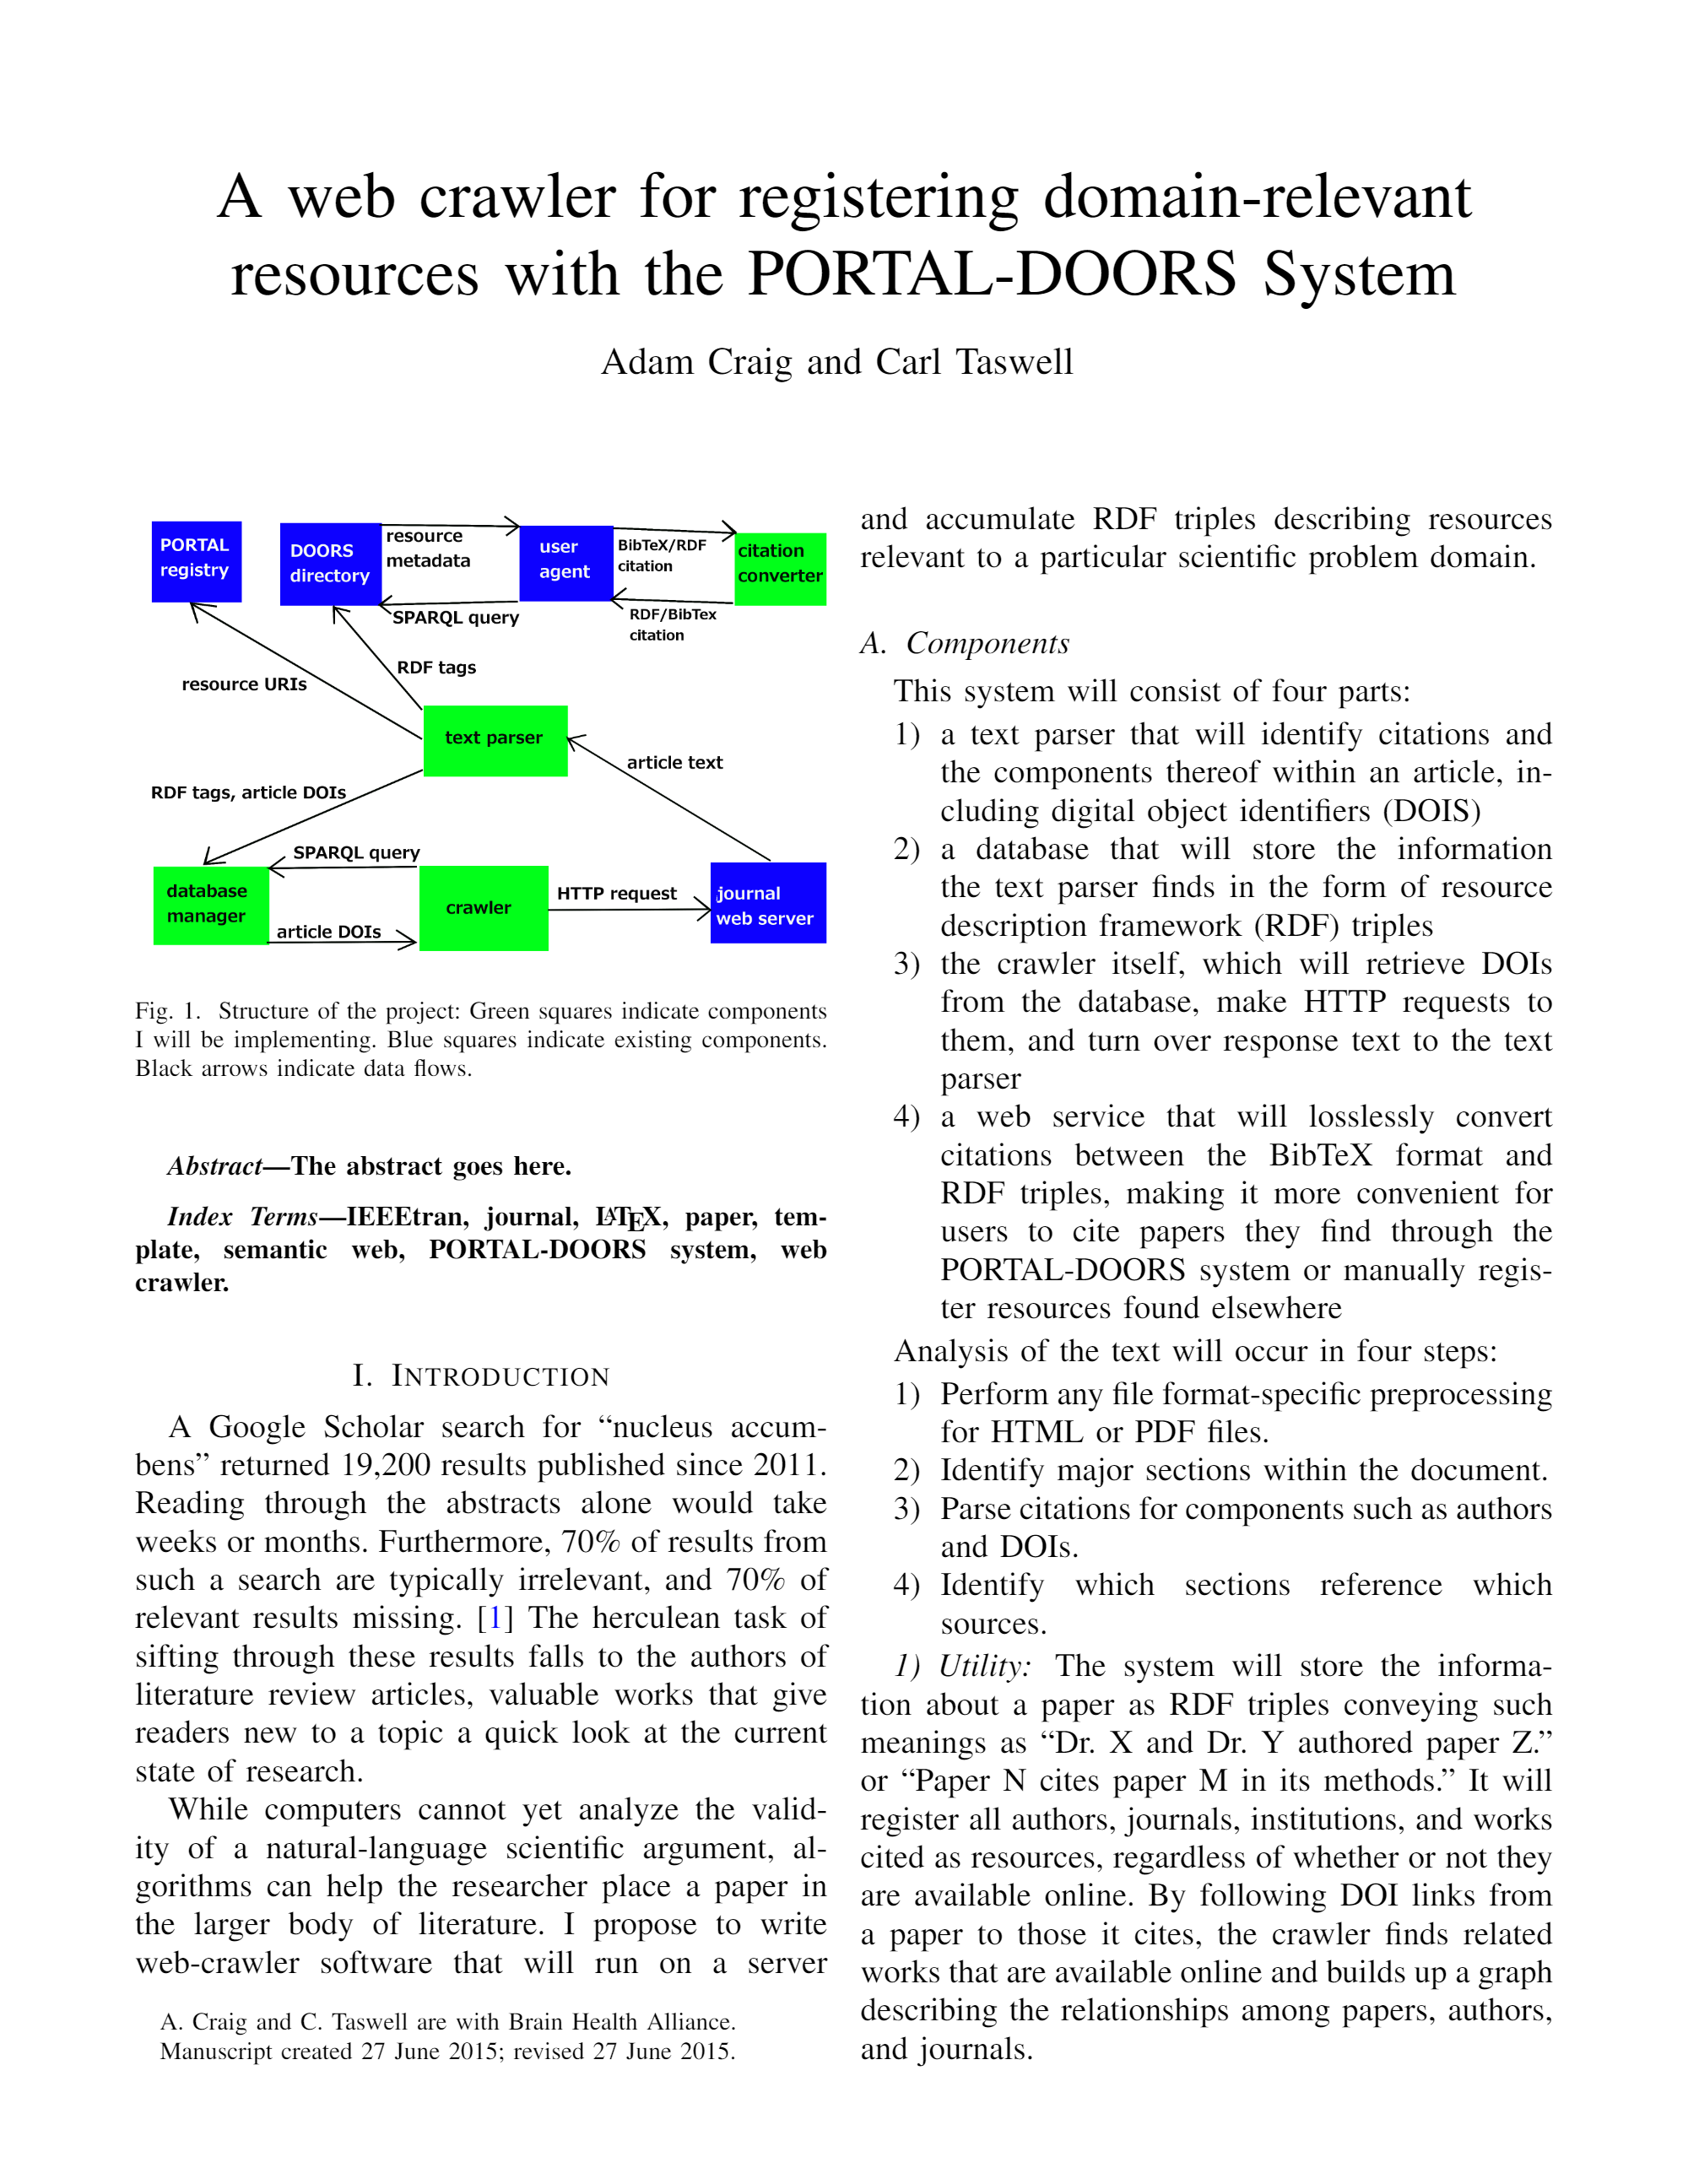
\includegraphics[scale=0.45]{NPDS_flowchart}	

	For this new NEXUS-PORTAL-DOORS (NPD) system implementation, MEAN (MongoDB, Express, Angular, Node.js)  stack is the most updated and contributed fullstack javascript framework. Both backend and front end will rely heavily on node.js, an open-source runtime environment which enables scalable web applications and servers. Used with Express and other packages, node.js enables the user to organize a web application into a MVC (model-view-controller) architecture. In accordance with the "M" from MEAN stack, MongoDB serves as the database for the NPD. As a noSQL database, MongoDB relies on collecetions and documents in contrast to tables and rows. However, MongoDB offers no implementation of queries or updates to the database. Mongoose, a popular object relational mapper for MongoDB, enables connection to a MongoDB database from javascript, allowing model abstraction, large scale queries, data validation, and more. It also enables the user to create schemas, which help generate a structured database. \newline
	
	In the NPDS system, Problem Oriented Registry of Tags And Labels (PORTAL) registers resource labels and tags, inserting or updating them into the database while the Domain Ontology Oriented Resource System (DOORS) publishes resource locations and descriptions with mapping of labels to locations for the semantic web, retrieving stored data from the database. Both PORTAl and DOORS can be optimized for faster read/write if organized in a heirarchical architecture. Within the database, the collections for each of these PORTAL, DOORS, AND NEXUS are named respectively with the prefixes pds P, pds D, and pds N. \newline

	In order to create this implementation of MongoDB and Mongoose for a NPDS system, a template is required as the starting platform. Working with other parts of the NPDS implementation, MongoDB will serve two purposes. One is to contain users for an authentication system, working alongside PassportJS. PassportJS enables the creation of accounts under username and password. It can also be implemented to receive authentication from third parties sucha s Facebook and Twitter, a common practice nowadays. However, for our purposes, the primary advantage of using passport is the level of flexibility it offers. Its primary goal is to keep the complexity of user authentication simple and done in as a few lines of code as possible. This is done with "strategies," which are modules which enable the user to specifically designate which form of authentication they desire, without uncessary modules. PassportJS also supports persistent sessions. Lastly, PassportJS enables the database to store the username as a string, but encodes the password with a series of numbers, ensuring a level of security for the user. The second purpose of MongoDB in the template is to read/write/store metadata. Although the collection names will be changed upon the generation of each server from the template, the role will not. The pimary purpose of the database in the PORTAL registrar is to be able to store metadata resources with labels and optional tags. Meanwhile, the in the DOORS directories, the database must be able to retrieve locations and descriptions of resources, which are specified by references to an OWL ontology.

August:
\begin{itemize}
	\item Week 3: Fix Mongoose query problems; Finish assembling template with all components; begin generating webpages for NPDS read registrar, NPDS write registrar, NEXUS read-only directory, PORTAL read-only registry, DOORS read-only directory
	\item Week 4: Conversion over to typescirpt; Individualize databases for each generated page; bug fixes
\end{itemize}
	

\section*{Results}
	The implementation of MongoDB for NPDS is a partial success. Currently, writing to the registrar is done smoothly in Mongoose. Storing XML data is also a success, being enabled by the npm module xml2js. However, retrievel through queries is currently still an issue. 


\section*{Discussion}
	Due to the flexbility of noSQL and especially lMongoDB's document based database, it offers a database storage which fit the purposes of storing metadata. Furthermore, the automation of this process is enabled by Mongoose, which also helps create a schema and acts as an ORM. The currently implementation proves the potential for a noSQL database such as MongoDB to play a role in the future of NPDS or other semantic web systems. 


\section*{Conclusion}
\label{secConclusion}
conclusion text here


\section*{Acknowledgments}
This research was supported by the Brain Health Alliance Virtual Institute. We'd like to thank everyone who particpated in the 2016 program with us, especially Sujay Ratna and Ben Bae, who worked with us toward a semantic web solution. 


\section*{References}
\begin{enumerate}
\item Barrasa Rodriguez, J., Corcho, �. and G�mez-P�rez, A.
R2O, an extensible and semantically based database-to-ontology mapping language
Springer-Verlag, 2004
\item Berners-Lee, T., Hendler, J., Lassila, O. and others
The semantic web
Scientific american, New York, NY, USA:, 2001, Vol. 284(5), pp. 28-37
\item Dickey, J.
Write modern web apps with the MEAN stack: Mongo, Express, AngularJS, and Node. js
Pearson Education, 2014
\item MySQL, A.
MySQL
2001
\item Pan, Z. and Heflin, J.
Dldb: Extending relational databases to support semantic web queries
DTIC Document, DTIC Document, 2004
\item Spanos, D.-E., Stavrou, P. and Mitrou, N.
Bringing relational databases into the semantic web: A survey
Semantic Web, IOS Press, 2012, Vol. 3(2), pp. 169-209
\item Stojanovic, L., Stojanovic, N. and Volz, R.
Migrating data-intensive web sites into the semantic web
Proceedings of the 2002 ACM symposium on Applied computing
2002, pp. 1100-1107
\item Suehring, S.
MySQL bible
John Wiley and Sons, Inc., 2002
\item Taswell, C.
DOORS to the semantic web and grid with a PORTAL for biomedical computing
IEEE Transactions on Information Technology in Biomedicine, IEEE, 2008, Vol. 12(2), pp. 191-204
\item Taswell, C.
Portals and doors for the semantic web and grid
Google Patents, 2010
\item Taswell, C.
A distributed infrastructure for metadata about metadata: The HDMM architectural style and PORTAL-DOORS system
Future Internet, Molecular Diversity Preservation International, 2010, Vol. 2(2), pp. 156-189
\end{enumerate}


% References: note that the \nocite{*} command will automatically generate 
%  a reference list for all references contained in all *.bib files separated by
%  commas in the \bibliography{} command.
\nocite{*}
\bibliographystyle{plainnat}
\bibliography{BrainWarping}
\end{document}